% Created by tikzDevice version 0.12.3.1 on 2021-10-17 10:40:53
% !TEX encoding = UTF-8 Unicode
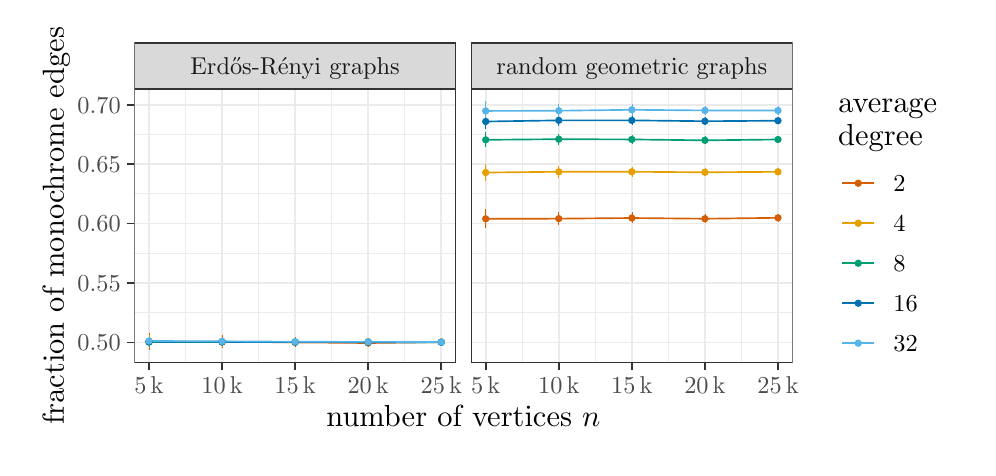
\begin{tikzpicture}[x=1pt,y=1pt]
\definecolor{fillColor}{RGB}{255,255,255}
\path[use as bounding box,fill=fillColor,fill opacity=0.00] (0,0) rectangle (339.67,151.77);
\begin{scope}
\path[clip] (  0.00,  0.00) rectangle (339.67,151.77);
\definecolor{drawColor}{RGB}{255,255,255}
\definecolor{fillColor}{RGB}{255,255,255}

\path[draw=drawColor,line width= 0.6pt,line join=round,line cap=round,fill=fillColor] (  0.00,  0.00) rectangle (339.67,151.77);
\end{scope}
\begin{scope}
\path[clip] ( 38.56, 30.69) rectangle (154.73,129.70);
\definecolor{fillColor}{RGB}{255,255,255}

\path[fill=fillColor] ( 38.56, 30.69) rectangle (154.73,129.70);
\definecolor{drawColor}{gray}{0.92}

\path[draw=drawColor,line width= 0.3pt,line join=round] ( 38.56, 48.78) --
	(154.73, 48.78);

\path[draw=drawColor,line width= 0.3pt,line join=round] ( 38.56, 70.24) --
	(154.73, 70.24);

\path[draw=drawColor,line width= 0.3pt,line join=round] ( 38.56, 91.70) --
	(154.73, 91.70);

\path[draw=drawColor,line width= 0.3pt,line join=round] ( 38.56,113.16) --
	(154.73,113.16);

\path[draw=drawColor,line width= 0.3pt,line join=round] ( 57.04, 30.69) --
	( 57.04,129.70);

\path[draw=drawColor,line width= 0.3pt,line join=round] ( 83.44, 30.69) --
	( 83.44,129.70);

\path[draw=drawColor,line width= 0.3pt,line join=round] (109.84, 30.69) --
	(109.84,129.70);

\path[draw=drawColor,line width= 0.3pt,line join=round] (136.24, 30.69) --
	(136.24,129.70);

\path[draw=drawColor,line width= 0.6pt,line join=round] ( 38.56, 38.05) --
	(154.73, 38.05);

\path[draw=drawColor,line width= 0.6pt,line join=round] ( 38.56, 59.51) --
	(154.73, 59.51);

\path[draw=drawColor,line width= 0.6pt,line join=round] ( 38.56, 80.97) --
	(154.73, 80.97);

\path[draw=drawColor,line width= 0.6pt,line join=round] ( 38.56,102.43) --
	(154.73,102.43);

\path[draw=drawColor,line width= 0.6pt,line join=round] ( 38.56,123.89) --
	(154.73,123.89);

\path[draw=drawColor,line width= 0.6pt,line join=round] ( 43.84, 30.69) --
	( 43.84,129.70);

\path[draw=drawColor,line width= 0.6pt,line join=round] ( 70.24, 30.69) --
	( 70.24,129.70);

\path[draw=drawColor,line width= 0.6pt,line join=round] ( 96.64, 30.69) --
	( 96.64,129.70);

\path[draw=drawColor,line width= 0.6pt,line join=round] (123.04, 30.69) --
	(123.04,129.70);

\path[draw=drawColor,line width= 0.6pt,line join=round] (149.45, 30.69) --
	(149.45,129.70);
\definecolor{drawColor}{RGB}{213,94,0}

\path[draw=drawColor,line width= 0.2pt,line join=round] ( 43.84, 41.47) --
	( 43.84, 41.47);

\path[draw=drawColor,line width= 0.2pt,line join=round] ( 43.84, 41.47) --
	( 43.84, 35.19);

\path[draw=drawColor,line width= 0.2pt,line join=round] ( 43.84, 35.19) --
	( 43.84, 35.19);

\path[draw=drawColor,line width= 0.2pt,line join=round] ( 70.24, 40.56) --
	( 70.24, 40.56);

\path[draw=drawColor,line width= 0.2pt,line join=round] ( 70.24, 40.56) --
	( 70.24, 35.94);

\path[draw=drawColor,line width= 0.2pt,line join=round] ( 70.24, 35.94) --
	( 70.24, 35.94);

\path[draw=drawColor,line width= 0.2pt,line join=round] ( 96.64, 39.86) --
	( 96.64, 39.86);

\path[draw=drawColor,line width= 0.2pt,line join=round] ( 96.64, 39.86) --
	( 96.64, 36.42);

\path[draw=drawColor,line width= 0.2pt,line join=round] ( 96.64, 36.42) --
	( 96.64, 36.42);

\path[draw=drawColor,line width= 0.2pt,line join=round] (123.04, 39.63) --
	(123.04, 39.63);

\path[draw=drawColor,line width= 0.2pt,line join=round] (123.04, 39.63) --
	(123.04, 36.33);

\path[draw=drawColor,line width= 0.2pt,line join=round] (123.04, 36.33) --
	(123.04, 36.33);

\path[draw=drawColor,line width= 0.2pt,line join=round] (149.45, 39.62) --
	(149.45, 39.62);

\path[draw=drawColor,line width= 0.2pt,line join=round] (149.45, 39.62) --
	(149.45, 36.60);

\path[draw=drawColor,line width= 0.2pt,line join=round] (149.45, 36.60) --
	(149.45, 36.60);
\definecolor{drawColor}{RGB}{230,159,0}

\path[draw=drawColor,line width= 0.2pt,line join=round] ( 43.84, 40.60) --
	( 43.84, 40.60);

\path[draw=drawColor,line width= 0.2pt,line join=round] ( 43.84, 40.60) --
	( 43.84, 36.15);

\path[draw=drawColor,line width= 0.2pt,line join=round] ( 43.84, 36.15) --
	( 43.84, 36.15);

\path[draw=drawColor,line width= 0.2pt,line join=round] ( 70.24, 39.75) --
	( 70.24, 39.75);

\path[draw=drawColor,line width= 0.2pt,line join=round] ( 70.24, 39.75) --
	( 70.24, 36.40);

\path[draw=drawColor,line width= 0.2pt,line join=round] ( 70.24, 36.40) --
	( 70.24, 36.40);

\path[draw=drawColor,line width= 0.2pt,line join=round] ( 96.64, 39.42) --
	( 96.64, 39.42);

\path[draw=drawColor,line width= 0.2pt,line join=round] ( 96.64, 39.42) --
	( 96.64, 36.72);

\path[draw=drawColor,line width= 0.2pt,line join=round] ( 96.64, 36.72) --
	( 96.64, 36.72);

\path[draw=drawColor,line width= 0.2pt,line join=round] (123.04, 39.41) --
	(123.04, 39.41);

\path[draw=drawColor,line width= 0.2pt,line join=round] (123.04, 39.41) --
	(123.04, 36.88);

\path[draw=drawColor,line width= 0.2pt,line join=round] (123.04, 36.88) --
	(123.04, 36.88);

\path[draw=drawColor,line width= 0.2pt,line join=round] (149.45, 39.21) --
	(149.45, 39.21);

\path[draw=drawColor,line width= 0.2pt,line join=round] (149.45, 39.21) --
	(149.45, 37.12);

\path[draw=drawColor,line width= 0.2pt,line join=round] (149.45, 37.12) --
	(149.45, 37.12);
\definecolor{drawColor}{RGB}{0,158,115}

\path[draw=drawColor,line width= 0.2pt,line join=round] ( 43.84, 39.97) --
	( 43.84, 39.97);

\path[draw=drawColor,line width= 0.2pt,line join=round] ( 43.84, 39.97) --
	( 43.84, 36.29);

\path[draw=drawColor,line width= 0.2pt,line join=round] ( 43.84, 36.29) --
	( 43.84, 36.29);

\path[draw=drawColor,line width= 0.2pt,line join=round] ( 70.24, 39.46) --
	( 70.24, 39.46);

\path[draw=drawColor,line width= 0.2pt,line join=round] ( 70.24, 39.46) --
	( 70.24, 36.86);

\path[draw=drawColor,line width= 0.2pt,line join=round] ( 70.24, 36.86) --
	( 70.24, 36.86);

\path[draw=drawColor,line width= 0.2pt,line join=round] ( 96.64, 39.05) --
	( 96.64, 39.05);

\path[draw=drawColor,line width= 0.2pt,line join=round] ( 96.64, 39.05) --
	( 96.64, 37.14);

\path[draw=drawColor,line width= 0.2pt,line join=round] ( 96.64, 37.14) --
	( 96.64, 37.14);

\path[draw=drawColor,line width= 0.2pt,line join=round] (123.04, 38.98) --
	(123.04, 38.98);

\path[draw=drawColor,line width= 0.2pt,line join=round] (123.04, 38.98) --
	(123.04, 37.33);

\path[draw=drawColor,line width= 0.2pt,line join=round] (123.04, 37.33) --
	(123.04, 37.33);

\path[draw=drawColor,line width= 0.2pt,line join=round] (149.45, 38.84) --
	(149.45, 38.84);

\path[draw=drawColor,line width= 0.2pt,line join=round] (149.45, 38.84) --
	(149.45, 37.33);

\path[draw=drawColor,line width= 0.2pt,line join=round] (149.45, 37.33) --
	(149.45, 37.33);
\definecolor{drawColor}{RGB}{0,114,178}

\path[draw=drawColor,line width= 0.2pt,line join=round] ( 43.84, 39.66) --
	( 43.84, 39.66);

\path[draw=drawColor,line width= 0.2pt,line join=round] ( 43.84, 39.66) --
	( 43.84, 36.96);

\path[draw=drawColor,line width= 0.2pt,line join=round] ( 43.84, 36.96) --
	( 43.84, 36.96);

\path[draw=drawColor,line width= 0.2pt,line join=round] ( 70.24, 39.17) --
	( 70.24, 39.17);

\path[draw=drawColor,line width= 0.2pt,line join=round] ( 70.24, 39.17) --
	( 70.24, 37.25);

\path[draw=drawColor,line width= 0.2pt,line join=round] ( 70.24, 37.25) --
	( 70.24, 37.25);

\path[draw=drawColor,line width= 0.2pt,line join=round] ( 96.64, 38.87) --
	( 96.64, 38.87);

\path[draw=drawColor,line width= 0.2pt,line join=round] ( 96.64, 38.87) --
	( 96.64, 37.43);

\path[draw=drawColor,line width= 0.2pt,line join=round] ( 96.64, 37.43) --
	( 96.64, 37.43);

\path[draw=drawColor,line width= 0.2pt,line join=round] (123.04, 38.65) --
	(123.04, 38.65);

\path[draw=drawColor,line width= 0.2pt,line join=round] (123.04, 38.65) --
	(123.04, 37.48);

\path[draw=drawColor,line width= 0.2pt,line join=round] (123.04, 37.48) --
	(123.04, 37.48);

\path[draw=drawColor,line width= 0.2pt,line join=round] (149.45, 38.69) --
	(149.45, 38.69);

\path[draw=drawColor,line width= 0.2pt,line join=round] (149.45, 38.69) --
	(149.45, 37.58);

\path[draw=drawColor,line width= 0.2pt,line join=round] (149.45, 37.58) --
	(149.45, 37.58);
\definecolor{drawColor}{RGB}{86,180,233}

\path[draw=drawColor,line width= 0.2pt,line join=round] ( 43.84, 39.72) --
	( 43.84, 39.72);

\path[draw=drawColor,line width= 0.2pt,line join=round] ( 43.84, 39.72) --
	( 43.84, 37.57);

\path[draw=drawColor,line width= 0.2pt,line join=round] ( 43.84, 37.57) --
	( 43.84, 37.57);

\path[draw=drawColor,line width= 0.2pt,line join=round] ( 70.24, 39.17) --
	( 70.24, 39.17);

\path[draw=drawColor,line width= 0.2pt,line join=round] ( 70.24, 39.17) --
	( 70.24, 37.71);

\path[draw=drawColor,line width= 0.2pt,line join=round] ( 70.24, 37.71) --
	( 70.24, 37.71);

\path[draw=drawColor,line width= 0.2pt,line join=round] ( 96.64, 38.85) --
	( 96.64, 38.85);

\path[draw=drawColor,line width= 0.2pt,line join=round] ( 96.64, 38.85) --
	( 96.64, 37.72);

\path[draw=drawColor,line width= 0.2pt,line join=round] ( 96.64, 37.72) --
	( 96.64, 37.72);

\path[draw=drawColor,line width= 0.2pt,line join=round] (123.04, 38.70) --
	(123.04, 38.70);

\path[draw=drawColor,line width= 0.2pt,line join=round] (123.04, 38.70) --
	(123.04, 37.73);

\path[draw=drawColor,line width= 0.2pt,line join=round] (123.04, 37.73) --
	(123.04, 37.73);

\path[draw=drawColor,line width= 0.2pt,line join=round] (149.45, 38.67) --
	(149.45, 38.67);

\path[draw=drawColor,line width= 0.2pt,line join=round] (149.45, 38.67) --
	(149.45, 37.77);

\path[draw=drawColor,line width= 0.2pt,line join=round] (149.45, 37.77) --
	(149.45, 37.77);
\definecolor{drawColor}{RGB}{213,94,0}

\path[draw=drawColor,line width= 0.6pt,line join=round] ( 43.84, 38.26) --
	( 70.24, 38.29) --
	( 96.64, 38.05) --
	(123.04, 37.82) --
	(149.45, 38.15);
\definecolor{drawColor}{RGB}{230,159,0}

\path[draw=drawColor,line width= 0.6pt,line join=round] ( 43.84, 38.19) --
	( 70.24, 38.16) --
	( 96.64, 38.12) --
	(123.04, 38.24) --
	(149.45, 38.23);
\definecolor{drawColor}{RGB}{0,158,115}

\path[draw=drawColor,line width= 0.6pt,line join=round] ( 43.84, 38.19) --
	( 70.24, 38.20) --
	( 96.64, 38.13) --
	(123.04, 38.16) --
	(149.45, 38.08);
\definecolor{drawColor}{RGB}{0,114,178}

\path[draw=drawColor,line width= 0.6pt,line join=round] ( 43.84, 38.28) --
	( 70.24, 38.22) --
	( 96.64, 38.16) --
	(123.04, 38.11) --
	(149.45, 38.13);
\definecolor{drawColor}{RGB}{86,180,233}

\path[draw=drawColor,line width= 0.6pt,line join=round] ( 43.84, 38.56) --
	( 70.24, 38.44) --
	( 96.64, 38.29) --
	(123.04, 38.22) --
	(149.45, 38.21);
\definecolor{drawColor}{RGB}{213,94,0}
\definecolor{fillColor}{RGB}{213,94,0}

\path[draw=drawColor,line width= 0.4pt,line join=round,line cap=round,fill=fillColor] ( 43.84, 38.26) circle (  1.11);

\path[draw=drawColor,line width= 0.4pt,line join=round,line cap=round,fill=fillColor] ( 70.24, 38.29) circle (  1.11);

\path[draw=drawColor,line width= 0.4pt,line join=round,line cap=round,fill=fillColor] ( 96.64, 38.05) circle (  1.11);

\path[draw=drawColor,line width= 0.4pt,line join=round,line cap=round,fill=fillColor] (123.04, 37.82) circle (  1.11);

\path[draw=drawColor,line width= 0.4pt,line join=round,line cap=round,fill=fillColor] (149.45, 38.15) circle (  1.11);
\definecolor{drawColor}{RGB}{230,159,0}
\definecolor{fillColor}{RGB}{230,159,0}

\path[draw=drawColor,line width= 0.4pt,line join=round,line cap=round,fill=fillColor] ( 43.84, 38.19) circle (  1.11);

\path[draw=drawColor,line width= 0.4pt,line join=round,line cap=round,fill=fillColor] ( 70.24, 38.16) circle (  1.11);

\path[draw=drawColor,line width= 0.4pt,line join=round,line cap=round,fill=fillColor] ( 96.64, 38.12) circle (  1.11);

\path[draw=drawColor,line width= 0.4pt,line join=round,line cap=round,fill=fillColor] (123.04, 38.24) circle (  1.11);

\path[draw=drawColor,line width= 0.4pt,line join=round,line cap=round,fill=fillColor] (149.45, 38.23) circle (  1.11);
\definecolor{drawColor}{RGB}{0,158,115}
\definecolor{fillColor}{RGB}{0,158,115}

\path[draw=drawColor,line width= 0.4pt,line join=round,line cap=round,fill=fillColor] ( 43.84, 38.19) circle (  1.11);

\path[draw=drawColor,line width= 0.4pt,line join=round,line cap=round,fill=fillColor] ( 70.24, 38.20) circle (  1.11);

\path[draw=drawColor,line width= 0.4pt,line join=round,line cap=round,fill=fillColor] ( 96.64, 38.13) circle (  1.11);

\path[draw=drawColor,line width= 0.4pt,line join=round,line cap=round,fill=fillColor] (123.04, 38.16) circle (  1.11);

\path[draw=drawColor,line width= 0.4pt,line join=round,line cap=round,fill=fillColor] (149.45, 38.08) circle (  1.11);
\definecolor{drawColor}{RGB}{0,114,178}
\definecolor{fillColor}{RGB}{0,114,178}

\path[draw=drawColor,line width= 0.4pt,line join=round,line cap=round,fill=fillColor] ( 43.84, 38.28) circle (  1.11);

\path[draw=drawColor,line width= 0.4pt,line join=round,line cap=round,fill=fillColor] ( 70.24, 38.22) circle (  1.11);

\path[draw=drawColor,line width= 0.4pt,line join=round,line cap=round,fill=fillColor] ( 96.64, 38.16) circle (  1.11);

\path[draw=drawColor,line width= 0.4pt,line join=round,line cap=round,fill=fillColor] (123.04, 38.11) circle (  1.11);

\path[draw=drawColor,line width= 0.4pt,line join=round,line cap=round,fill=fillColor] (149.45, 38.13) circle (  1.11);
\definecolor{drawColor}{RGB}{86,180,233}
\definecolor{fillColor}{RGB}{86,180,233}

\path[draw=drawColor,line width= 0.4pt,line join=round,line cap=round,fill=fillColor] ( 43.84, 38.56) circle (  1.11);

\path[draw=drawColor,line width= 0.4pt,line join=round,line cap=round,fill=fillColor] ( 70.24, 38.44) circle (  1.11);

\path[draw=drawColor,line width= 0.4pt,line join=round,line cap=round,fill=fillColor] ( 96.64, 38.29) circle (  1.11);

\path[draw=drawColor,line width= 0.4pt,line join=round,line cap=round,fill=fillColor] (123.04, 38.22) circle (  1.11);

\path[draw=drawColor,line width= 0.4pt,line join=round,line cap=round,fill=fillColor] (149.45, 38.21) circle (  1.11);
\definecolor{drawColor}{gray}{0.20}

\path[draw=drawColor,line width= 0.6pt,line join=round,line cap=round] ( 38.56, 30.69) rectangle (154.73,129.70);
\end{scope}
\begin{scope}
\path[clip] (160.23, 30.69) rectangle (276.40,129.70);
\definecolor{fillColor}{RGB}{255,255,255}

\path[fill=fillColor] (160.23, 30.69) rectangle (276.40,129.70);
\definecolor{drawColor}{gray}{0.92}

\path[draw=drawColor,line width= 0.3pt,line join=round] (160.23, 48.78) --
	(276.40, 48.78);

\path[draw=drawColor,line width= 0.3pt,line join=round] (160.23, 70.24) --
	(276.40, 70.24);

\path[draw=drawColor,line width= 0.3pt,line join=round] (160.23, 91.70) --
	(276.40, 91.70);

\path[draw=drawColor,line width= 0.3pt,line join=round] (160.23,113.16) --
	(276.40,113.16);

\path[draw=drawColor,line width= 0.3pt,line join=round] (178.71, 30.69) --
	(178.71,129.70);

\path[draw=drawColor,line width= 0.3pt,line join=round] (205.11, 30.69) --
	(205.11,129.70);

\path[draw=drawColor,line width= 0.3pt,line join=round] (231.51, 30.69) --
	(231.51,129.70);

\path[draw=drawColor,line width= 0.3pt,line join=round] (257.92, 30.69) --
	(257.92,129.70);

\path[draw=drawColor,line width= 0.6pt,line join=round] (160.23, 38.05) --
	(276.40, 38.05);

\path[draw=drawColor,line width= 0.6pt,line join=round] (160.23, 59.51) --
	(276.40, 59.51);

\path[draw=drawColor,line width= 0.6pt,line join=round] (160.23, 80.97) --
	(276.40, 80.97);

\path[draw=drawColor,line width= 0.6pt,line join=round] (160.23,102.43) --
	(276.40,102.43);

\path[draw=drawColor,line width= 0.6pt,line join=round] (160.23,123.89) --
	(276.40,123.89);

\path[draw=drawColor,line width= 0.6pt,line join=round] (165.51, 30.69) --
	(165.51,129.70);

\path[draw=drawColor,line width= 0.6pt,line join=round] (191.91, 30.69) --
	(191.91,129.70);

\path[draw=drawColor,line width= 0.6pt,line join=round] (218.31, 30.69) --
	(218.31,129.70);

\path[draw=drawColor,line width= 0.6pt,line join=round] (244.71, 30.69) --
	(244.71,129.70);

\path[draw=drawColor,line width= 0.6pt,line join=round] (271.12, 30.69) --
	(271.12,129.70);
\definecolor{drawColor}{RGB}{213,94,0}

\path[draw=drawColor,line width= 0.2pt,line join=round] (165.51, 86.08) --
	(165.51, 86.08);

\path[draw=drawColor,line width= 0.2pt,line join=round] (165.51, 86.08) --
	(165.51, 79.49);

\path[draw=drawColor,line width= 0.2pt,line join=round] (165.51, 79.49) --
	(165.51, 79.49);

\path[draw=drawColor,line width= 0.2pt,line join=round] (191.91, 85.29) --
	(191.91, 85.29);

\path[draw=drawColor,line width= 0.2pt,line join=round] (191.91, 85.29) --
	(191.91, 80.41);

\path[draw=drawColor,line width= 0.2pt,line join=round] (191.91, 80.41) --
	(191.91, 80.41);

\path[draw=drawColor,line width= 0.2pt,line join=round] (218.31, 85.07) --
	(218.31, 85.07);

\path[draw=drawColor,line width= 0.2pt,line join=round] (218.31, 85.07) --
	(218.31, 81.06);

\path[draw=drawColor,line width= 0.2pt,line join=round] (218.31, 81.06) --
	(218.31, 81.06);

\path[draw=drawColor,line width= 0.2pt,line join=round] (244.71, 84.53) --
	(244.71, 84.53);

\path[draw=drawColor,line width= 0.2pt,line join=round] (244.71, 84.53) --
	(244.71, 81.22);

\path[draw=drawColor,line width= 0.2pt,line join=round] (244.71, 81.22) --
	(244.71, 81.22);

\path[draw=drawColor,line width= 0.2pt,line join=round] (271.12, 84.46) --
	(271.12, 84.46);

\path[draw=drawColor,line width= 0.2pt,line join=round] (271.12, 84.46) --
	(271.12, 81.60);

\path[draw=drawColor,line width= 0.2pt,line join=round] (271.12, 81.60) --
	(271.12, 81.60);
\definecolor{drawColor}{RGB}{230,159,0}

\path[draw=drawColor,line width= 0.2pt,line join=round] (165.51,102.46) --
	(165.51,102.46);

\path[draw=drawColor,line width= 0.2pt,line join=round] (165.51,102.46) --
	(165.51, 96.48);

\path[draw=drawColor,line width= 0.2pt,line join=round] (165.51, 96.48) --
	(165.51, 96.48);

\path[draw=drawColor,line width= 0.2pt,line join=round] (191.91,101.72) --
	(191.91,101.72);

\path[draw=drawColor,line width= 0.2pt,line join=round] (191.91,101.72) --
	(191.91, 97.55);

\path[draw=drawColor,line width= 0.2pt,line join=round] (191.91, 97.55) --
	(191.91, 97.55);

\path[draw=drawColor,line width= 0.2pt,line join=round] (218.31,101.26) --
	(218.31,101.26);

\path[draw=drawColor,line width= 0.2pt,line join=round] (218.31,101.26) --
	(218.31, 97.86);

\path[draw=drawColor,line width= 0.2pt,line join=round] (218.31, 97.86) --
	(218.31, 97.86);

\path[draw=drawColor,line width= 0.2pt,line join=round] (244.71,100.93) --
	(244.71,100.93);

\path[draw=drawColor,line width= 0.2pt,line join=round] (244.71,100.93) --
	(244.71, 98.09);

\path[draw=drawColor,line width= 0.2pt,line join=round] (244.71, 98.09) --
	(244.71, 98.09);

\path[draw=drawColor,line width= 0.2pt,line join=round] (271.12,101.07) --
	(271.12,101.07);

\path[draw=drawColor,line width= 0.2pt,line join=round] (271.12,101.07) --
	(271.12, 98.41);

\path[draw=drawColor,line width= 0.2pt,line join=round] (271.12, 98.41) --
	(271.12, 98.41);
\definecolor{drawColor}{RGB}{0,158,115}

\path[draw=drawColor,line width= 0.2pt,line join=round] (165.51,114.00) --
	(165.51,114.00);

\path[draw=drawColor,line width= 0.2pt,line join=round] (165.51,114.00) --
	(165.51,108.57);

\path[draw=drawColor,line width= 0.2pt,line join=round] (165.51,108.57) --
	(165.51,108.57);

\path[draw=drawColor,line width= 0.2pt,line join=round] (191.91,113.32) --
	(191.91,113.32);

\path[draw=drawColor,line width= 0.2pt,line join=round] (191.91,113.32) --
	(191.91,109.43);

\path[draw=drawColor,line width= 0.2pt,line join=round] (191.91,109.43) --
	(191.91,109.43);

\path[draw=drawColor,line width= 0.2pt,line join=round] (218.31,113.04) --
	(218.31,113.04);

\path[draw=drawColor,line width= 0.2pt,line join=round] (218.31,113.04) --
	(218.31,109.81);

\path[draw=drawColor,line width= 0.2pt,line join=round] (218.31,109.81) --
	(218.31,109.81);

\path[draw=drawColor,line width= 0.2pt,line join=round] (244.71,112.49) --
	(244.71,112.49);

\path[draw=drawColor,line width= 0.2pt,line join=round] (244.71,112.49) --
	(244.71,109.74);

\path[draw=drawColor,line width= 0.2pt,line join=round] (244.71,109.74) --
	(244.71,109.74);

\path[draw=drawColor,line width= 0.2pt,line join=round] (271.12,112.50) --
	(271.12,112.50);

\path[draw=drawColor,line width= 0.2pt,line join=round] (271.12,112.50) --
	(271.12,110.06);

\path[draw=drawColor,line width= 0.2pt,line join=round] (271.12,110.06) --
	(271.12,110.06);
\definecolor{drawColor}{RGB}{0,114,178}

\path[draw=drawColor,line width= 0.2pt,line join=round] (165.51,120.86) --
	(165.51,120.86);

\path[draw=drawColor,line width= 0.2pt,line join=round] (165.51,120.86) --
	(165.51,115.11);

\path[draw=drawColor,line width= 0.2pt,line join=round] (165.51,115.11) --
	(165.51,115.11);

\path[draw=drawColor,line width= 0.2pt,line join=round] (191.91,120.33) --
	(191.91,120.33);

\path[draw=drawColor,line width= 0.2pt,line join=round] (191.91,120.33) --
	(191.91,116.22);

\path[draw=drawColor,line width= 0.2pt,line join=round] (191.91,116.22) --
	(191.91,116.22);

\path[draw=drawColor,line width= 0.2pt,line join=round] (218.31,120.14) --
	(218.31,120.14);

\path[draw=drawColor,line width= 0.2pt,line join=round] (218.31,120.14) --
	(218.31,116.67);

\path[draw=drawColor,line width= 0.2pt,line join=round] (218.31,116.67) --
	(218.31,116.67);

\path[draw=drawColor,line width= 0.2pt,line join=round] (244.71,119.36) --
	(244.71,119.36);

\path[draw=drawColor,line width= 0.2pt,line join=round] (244.71,119.36) --
	(244.71,116.71);

\path[draw=drawColor,line width= 0.2pt,line join=round] (244.71,116.71) --
	(244.71,116.71);

\path[draw=drawColor,line width= 0.2pt,line join=round] (271.12,119.40) --
	(271.12,119.40);

\path[draw=drawColor,line width= 0.2pt,line join=round] (271.12,119.40) --
	(271.12,116.85);

\path[draw=drawColor,line width= 0.2pt,line join=round] (271.12,116.85) --
	(271.12,116.85);
\definecolor{drawColor}{RGB}{86,180,233}

\path[draw=drawColor,line width= 0.2pt,line join=round] (165.51,125.20) --
	(165.51,125.20);

\path[draw=drawColor,line width= 0.2pt,line join=round] (165.51,125.20) --
	(165.51,118.34);

\path[draw=drawColor,line width= 0.2pt,line join=round] (165.51,118.34) --
	(165.51,118.34);

\path[draw=drawColor,line width= 0.2pt,line join=round] (191.91,124.29) --
	(191.91,124.29);

\path[draw=drawColor,line width= 0.2pt,line join=round] (191.91,124.29) --
	(191.91,119.28);

\path[draw=drawColor,line width= 0.2pt,line join=round] (191.91,119.28) --
	(191.91,119.28);

\path[draw=drawColor,line width= 0.2pt,line join=round] (218.31,124.04) --
	(218.31,124.04);

\path[draw=drawColor,line width= 0.2pt,line join=round] (218.31,124.04) --
	(218.31,120.01);

\path[draw=drawColor,line width= 0.2pt,line join=round] (218.31,120.01) --
	(218.31,120.01);

\path[draw=drawColor,line width= 0.2pt,line join=round] (244.71,123.54) --
	(244.71,123.54);

\path[draw=drawColor,line width= 0.2pt,line join=round] (244.71,123.54) --
	(244.71,120.12);

\path[draw=drawColor,line width= 0.2pt,line join=round] (244.71,120.12) --
	(244.71,120.12);

\path[draw=drawColor,line width= 0.2pt,line join=round] (271.12,123.32) --
	(271.12,123.32);

\path[draw=drawColor,line width= 0.2pt,line join=round] (271.12,123.32) --
	(271.12,120.22);

\path[draw=drawColor,line width= 0.2pt,line join=round] (271.12,120.22) --
	(271.12,120.22);
\definecolor{drawColor}{RGB}{213,94,0}

\path[draw=drawColor,line width= 0.6pt,line join=round] (165.51, 82.70) --
	(191.91, 82.76) --
	(218.31, 82.99) --
	(244.71, 82.73) --
	(271.12, 83.06);
\definecolor{drawColor}{RGB}{230,159,0}

\path[draw=drawColor,line width= 0.6pt,line join=round] (165.51, 99.42) --
	(191.91, 99.70) --
	(218.31, 99.70) --
	(244.71, 99.51) --
	(271.12, 99.68);
\definecolor{drawColor}{RGB}{0,158,115}

\path[draw=drawColor,line width= 0.6pt,line join=round] (165.51,111.25) --
	(191.91,111.47) --
	(218.31,111.38) --
	(244.71,111.06) --
	(271.12,111.36);
\definecolor{drawColor}{RGB}{0,114,178}

\path[draw=drawColor,line width= 0.6pt,line join=round] (165.51,117.86) --
	(191.91,118.27) --
	(218.31,118.27) --
	(244.71,117.97) --
	(271.12,118.15);
\definecolor{drawColor}{RGB}{86,180,233}

\path[draw=drawColor,line width= 0.6pt,line join=round] (165.51,121.68) --
	(191.91,121.76) --
	(218.31,122.09) --
	(244.71,121.86) --
	(271.12,121.83);
\definecolor{drawColor}{RGB}{213,94,0}
\definecolor{fillColor}{RGB}{213,94,0}

\path[draw=drawColor,line width= 0.4pt,line join=round,line cap=round,fill=fillColor] (165.51, 82.70) circle (  1.11);

\path[draw=drawColor,line width= 0.4pt,line join=round,line cap=round,fill=fillColor] (191.91, 82.76) circle (  1.11);

\path[draw=drawColor,line width= 0.4pt,line join=round,line cap=round,fill=fillColor] (218.31, 82.99) circle (  1.11);

\path[draw=drawColor,line width= 0.4pt,line join=round,line cap=round,fill=fillColor] (244.71, 82.73) circle (  1.11);

\path[draw=drawColor,line width= 0.4pt,line join=round,line cap=round,fill=fillColor] (271.12, 83.06) circle (  1.11);
\definecolor{drawColor}{RGB}{230,159,0}
\definecolor{fillColor}{RGB}{230,159,0}

\path[draw=drawColor,line width= 0.4pt,line join=round,line cap=round,fill=fillColor] (165.51, 99.42) circle (  1.11);

\path[draw=drawColor,line width= 0.4pt,line join=round,line cap=round,fill=fillColor] (191.91, 99.70) circle (  1.11);

\path[draw=drawColor,line width= 0.4pt,line join=round,line cap=round,fill=fillColor] (218.31, 99.70) circle (  1.11);

\path[draw=drawColor,line width= 0.4pt,line join=round,line cap=round,fill=fillColor] (244.71, 99.51) circle (  1.11);

\path[draw=drawColor,line width= 0.4pt,line join=round,line cap=round,fill=fillColor] (271.12, 99.68) circle (  1.11);
\definecolor{drawColor}{RGB}{0,158,115}
\definecolor{fillColor}{RGB}{0,158,115}

\path[draw=drawColor,line width= 0.4pt,line join=round,line cap=round,fill=fillColor] (165.51,111.25) circle (  1.11);

\path[draw=drawColor,line width= 0.4pt,line join=round,line cap=round,fill=fillColor] (191.91,111.47) circle (  1.11);

\path[draw=drawColor,line width= 0.4pt,line join=round,line cap=round,fill=fillColor] (218.31,111.38) circle (  1.11);

\path[draw=drawColor,line width= 0.4pt,line join=round,line cap=round,fill=fillColor] (244.71,111.06) circle (  1.11);

\path[draw=drawColor,line width= 0.4pt,line join=round,line cap=round,fill=fillColor] (271.12,111.36) circle (  1.11);
\definecolor{drawColor}{RGB}{0,114,178}
\definecolor{fillColor}{RGB}{0,114,178}

\path[draw=drawColor,line width= 0.4pt,line join=round,line cap=round,fill=fillColor] (165.51,117.86) circle (  1.11);

\path[draw=drawColor,line width= 0.4pt,line join=round,line cap=round,fill=fillColor] (191.91,118.27) circle (  1.11);

\path[draw=drawColor,line width= 0.4pt,line join=round,line cap=round,fill=fillColor] (218.31,118.27) circle (  1.11);

\path[draw=drawColor,line width= 0.4pt,line join=round,line cap=round,fill=fillColor] (244.71,117.97) circle (  1.11);

\path[draw=drawColor,line width= 0.4pt,line join=round,line cap=round,fill=fillColor] (271.12,118.15) circle (  1.11);
\definecolor{drawColor}{RGB}{86,180,233}
\definecolor{fillColor}{RGB}{86,180,233}

\path[draw=drawColor,line width= 0.4pt,line join=round,line cap=round,fill=fillColor] (165.51,121.68) circle (  1.11);

\path[draw=drawColor,line width= 0.4pt,line join=round,line cap=round,fill=fillColor] (191.91,121.76) circle (  1.11);

\path[draw=drawColor,line width= 0.4pt,line join=round,line cap=round,fill=fillColor] (218.31,122.09) circle (  1.11);

\path[draw=drawColor,line width= 0.4pt,line join=round,line cap=round,fill=fillColor] (244.71,121.86) circle (  1.11);

\path[draw=drawColor,line width= 0.4pt,line join=round,line cap=round,fill=fillColor] (271.12,121.83) circle (  1.11);
\definecolor{drawColor}{gray}{0.20}

\path[draw=drawColor,line width= 0.6pt,line join=round,line cap=round] (160.23, 30.69) rectangle (276.40,129.70);
\end{scope}
\begin{scope}
\path[clip] ( 38.56,129.70) rectangle (154.73,146.27);
\definecolor{drawColor}{gray}{0.20}
\definecolor{fillColor}{gray}{0.85}

\path[draw=drawColor,line width= 0.6pt,line join=round,line cap=round,fill=fillColor] ( 38.56,129.70) rectangle (154.73,146.27);
\definecolor{drawColor}{gray}{0.10}

\node[text=drawColor,anchor=base,inner sep=0pt, outer sep=0pt, scale=  0.88] at ( 96.64,134.95) {Erd{\H o}s-R\'enyi graphs};
\end{scope}
\begin{scope}
\path[clip] (160.23,129.70) rectangle (276.40,146.27);
\definecolor{drawColor}{gray}{0.20}
\definecolor{fillColor}{gray}{0.85}

\path[draw=drawColor,line width= 0.6pt,line join=round,line cap=round,fill=fillColor] (160.23,129.70) rectangle (276.40,146.27);
\definecolor{drawColor}{gray}{0.10}

\node[text=drawColor,anchor=base,inner sep=0pt, outer sep=0pt, scale=  0.88] at (218.31,134.95) {random geometric graphs};
\end{scope}
\begin{scope}
\path[clip] (  0.00,  0.00) rectangle (339.67,151.77);
\definecolor{drawColor}{gray}{0.20}

\path[draw=drawColor,line width= 0.6pt,line join=round] ( 43.84, 27.94) --
	( 43.84, 30.69);

\path[draw=drawColor,line width= 0.6pt,line join=round] ( 70.24, 27.94) --
	( 70.24, 30.69);

\path[draw=drawColor,line width= 0.6pt,line join=round] ( 96.64, 27.94) --
	( 96.64, 30.69);

\path[draw=drawColor,line width= 0.6pt,line join=round] (123.04, 27.94) --
	(123.04, 30.69);

\path[draw=drawColor,line width= 0.6pt,line join=round] (149.45, 27.94) --
	(149.45, 30.69);
\end{scope}
\begin{scope}
\path[clip] (  0.00,  0.00) rectangle (339.67,151.77);
\definecolor{drawColor}{gray}{0.30}

\node[text=drawColor,anchor=base,inner sep=0pt, outer sep=0pt, scale=  0.88] at ( 43.84, 19.68) {5\,k};

\node[text=drawColor,anchor=base,inner sep=0pt, outer sep=0pt, scale=  0.88] at ( 70.24, 19.68) {10\,k};

\node[text=drawColor,anchor=base,inner sep=0pt, outer sep=0pt, scale=  0.88] at ( 96.64, 19.68) {15\,k};

\node[text=drawColor,anchor=base,inner sep=0pt, outer sep=0pt, scale=  0.88] at (123.04, 19.68) {20\,k};

\node[text=drawColor,anchor=base,inner sep=0pt, outer sep=0pt, scale=  0.88] at (149.45, 19.68) {25\,k};
\end{scope}
\begin{scope}
\path[clip] (  0.00,  0.00) rectangle (339.67,151.77);
\definecolor{drawColor}{gray}{0.20}

\path[draw=drawColor,line width= 0.6pt,line join=round] (165.51, 27.94) --
	(165.51, 30.69);

\path[draw=drawColor,line width= 0.6pt,line join=round] (191.91, 27.94) --
	(191.91, 30.69);

\path[draw=drawColor,line width= 0.6pt,line join=round] (218.31, 27.94) --
	(218.31, 30.69);

\path[draw=drawColor,line width= 0.6pt,line join=round] (244.71, 27.94) --
	(244.71, 30.69);

\path[draw=drawColor,line width= 0.6pt,line join=round] (271.12, 27.94) --
	(271.12, 30.69);
\end{scope}
\begin{scope}
\path[clip] (  0.00,  0.00) rectangle (339.67,151.77);
\definecolor{drawColor}{gray}{0.30}

\node[text=drawColor,anchor=base,inner sep=0pt, outer sep=0pt, scale=  0.88] at (165.51, 19.68) {5\,k};

\node[text=drawColor,anchor=base,inner sep=0pt, outer sep=0pt, scale=  0.88] at (191.91, 19.68) {10\,k};

\node[text=drawColor,anchor=base,inner sep=0pt, outer sep=0pt, scale=  0.88] at (218.31, 19.68) {15\,k};

\node[text=drawColor,anchor=base,inner sep=0pt, outer sep=0pt, scale=  0.88] at (244.71, 19.68) {20\,k};

\node[text=drawColor,anchor=base,inner sep=0pt, outer sep=0pt, scale=  0.88] at (271.12, 19.68) {25\,k};
\end{scope}
\begin{scope}
\path[clip] (  0.00,  0.00) rectangle (339.67,151.77);
\definecolor{drawColor}{gray}{0.30}

\node[text=drawColor,anchor=base east,inner sep=0pt, outer sep=0pt, scale=  0.88] at ( 33.61, 35.02) {0.50};

\node[text=drawColor,anchor=base east,inner sep=0pt, outer sep=0pt, scale=  0.88] at ( 33.61, 56.48) {0.55};

\node[text=drawColor,anchor=base east,inner sep=0pt, outer sep=0pt, scale=  0.88] at ( 33.61, 77.94) {0.60};

\node[text=drawColor,anchor=base east,inner sep=0pt, outer sep=0pt, scale=  0.88] at ( 33.61, 99.40) {0.65};

\node[text=drawColor,anchor=base east,inner sep=0pt, outer sep=0pt, scale=  0.88] at ( 33.61,120.86) {0.70};
\end{scope}
\begin{scope}
\path[clip] (  0.00,  0.00) rectangle (339.67,151.77);
\definecolor{drawColor}{gray}{0.20}

\path[draw=drawColor,line width= 0.6pt,line join=round] ( 35.81, 38.05) --
	( 38.56, 38.05);

\path[draw=drawColor,line width= 0.6pt,line join=round] ( 35.81, 59.51) --
	( 38.56, 59.51);

\path[draw=drawColor,line width= 0.6pt,line join=round] ( 35.81, 80.97) --
	( 38.56, 80.97);

\path[draw=drawColor,line width= 0.6pt,line join=round] ( 35.81,102.43) --
	( 38.56,102.43);

\path[draw=drawColor,line width= 0.6pt,line join=round] ( 35.81,123.89) --
	( 38.56,123.89);
\end{scope}
\begin{scope}
\path[clip] (  0.00,  0.00) rectangle (339.67,151.77);
\definecolor{drawColor}{RGB}{0,0,0}

\node[text=drawColor,anchor=base,inner sep=0pt, outer sep=0pt, scale=  1.10] at (157.48,  7.64) {number of vertices $n$};
\end{scope}
\begin{scope}
\path[clip] (  0.00,  0.00) rectangle (339.67,151.77);
\definecolor{drawColor}{RGB}{0,0,0}

\node[text=drawColor,rotate= 90.00,anchor=base,inner sep=0pt, outer sep=0pt, scale=  1.10] at ( 13.08, 80.19) {fraction of monochrome edges};
\end{scope}
\begin{scope}
\path[clip] (  0.00,  0.00) rectangle (339.67,151.77);
\definecolor{fillColor}{RGB}{255,255,255}

\path[fill=fillColor] (287.40, 25.01) rectangle (334.17,135.37);
\end{scope}
\begin{scope}
\path[clip] (  0.00,  0.00) rectangle (339.67,151.77);
\definecolor{drawColor}{RGB}{0,0,0}

\node[text=drawColor,anchor=base west,inner sep=0pt, outer sep=0pt, scale=  1.10] at (292.90,121.23) {average};

\node[text=drawColor,anchor=base west,inner sep=0pt, outer sep=0pt, scale=  1.10] at (292.90,109.35) {degree};
\end{scope}
\begin{scope}
\path[clip] (  0.00,  0.00) rectangle (339.67,151.77);
\definecolor{fillColor}{RGB}{255,255,255}

\path[fill=fillColor] (292.90, 88.32) rectangle (307.35,102.78);
\end{scope}
\begin{scope}
\path[clip] (  0.00,  0.00) rectangle (339.67,151.77);
\definecolor{drawColor}{RGB}{213,94,0}

\path[draw=drawColor,line width= 0.2pt,line join=round] (294.34, 95.55) -- (305.91, 95.55);
\end{scope}
\begin{scope}
\path[clip] (  0.00,  0.00) rectangle (339.67,151.77);
\definecolor{drawColor}{RGB}{213,94,0}

\path[draw=drawColor,line width= 0.6pt,line join=round] (294.34, 95.55) -- (305.91, 95.55);
\end{scope}
\begin{scope}
\path[clip] (  0.00,  0.00) rectangle (339.67,151.77);
\definecolor{drawColor}{RGB}{213,94,0}
\definecolor{fillColor}{RGB}{213,94,0}

\path[draw=drawColor,line width= 0.4pt,line join=round,line cap=round,fill=fillColor] (300.12, 95.55) circle (  1.11);
\end{scope}
\begin{scope}
\path[clip] (  0.00,  0.00) rectangle (339.67,151.77);
\definecolor{fillColor}{RGB}{255,255,255}

\path[fill=fillColor] (292.90, 73.87) rectangle (307.35, 88.32);
\end{scope}
\begin{scope}
\path[clip] (  0.00,  0.00) rectangle (339.67,151.77);
\definecolor{drawColor}{RGB}{230,159,0}

\path[draw=drawColor,line width= 0.2pt,line join=round] (294.34, 81.10) -- (305.91, 81.10);
\end{scope}
\begin{scope}
\path[clip] (  0.00,  0.00) rectangle (339.67,151.77);
\definecolor{drawColor}{RGB}{230,159,0}

\path[draw=drawColor,line width= 0.6pt,line join=round] (294.34, 81.10) -- (305.91, 81.10);
\end{scope}
\begin{scope}
\path[clip] (  0.00,  0.00) rectangle (339.67,151.77);
\definecolor{drawColor}{RGB}{230,159,0}
\definecolor{fillColor}{RGB}{230,159,0}

\path[draw=drawColor,line width= 0.4pt,line join=round,line cap=round,fill=fillColor] (300.12, 81.10) circle (  1.11);
\end{scope}
\begin{scope}
\path[clip] (  0.00,  0.00) rectangle (339.67,151.77);
\definecolor{fillColor}{RGB}{255,255,255}

\path[fill=fillColor] (292.90, 59.42) rectangle (307.35, 73.87);
\end{scope}
\begin{scope}
\path[clip] (  0.00,  0.00) rectangle (339.67,151.77);
\definecolor{drawColor}{RGB}{0,158,115}

\path[draw=drawColor,line width= 0.2pt,line join=round] (294.34, 66.64) -- (305.91, 66.64);
\end{scope}
\begin{scope}
\path[clip] (  0.00,  0.00) rectangle (339.67,151.77);
\definecolor{drawColor}{RGB}{0,158,115}

\path[draw=drawColor,line width= 0.6pt,line join=round] (294.34, 66.64) -- (305.91, 66.64);
\end{scope}
\begin{scope}
\path[clip] (  0.00,  0.00) rectangle (339.67,151.77);
\definecolor{drawColor}{RGB}{0,158,115}
\definecolor{fillColor}{RGB}{0,158,115}

\path[draw=drawColor,line width= 0.4pt,line join=round,line cap=round,fill=fillColor] (300.12, 66.64) circle (  1.11);
\end{scope}
\begin{scope}
\path[clip] (  0.00,  0.00) rectangle (339.67,151.77);
\definecolor{fillColor}{RGB}{255,255,255}

\path[fill=fillColor] (292.90, 44.96) rectangle (307.35, 59.42);
\end{scope}
\begin{scope}
\path[clip] (  0.00,  0.00) rectangle (339.67,151.77);
\definecolor{drawColor}{RGB}{0,114,178}

\path[draw=drawColor,line width= 0.2pt,line join=round] (294.34, 52.19) -- (305.91, 52.19);
\end{scope}
\begin{scope}
\path[clip] (  0.00,  0.00) rectangle (339.67,151.77);
\definecolor{drawColor}{RGB}{0,114,178}

\path[draw=drawColor,line width= 0.6pt,line join=round] (294.34, 52.19) -- (305.91, 52.19);
\end{scope}
\begin{scope}
\path[clip] (  0.00,  0.00) rectangle (339.67,151.77);
\definecolor{drawColor}{RGB}{0,114,178}
\definecolor{fillColor}{RGB}{0,114,178}

\path[draw=drawColor,line width= 0.4pt,line join=round,line cap=round,fill=fillColor] (300.12, 52.19) circle (  1.11);
\end{scope}
\begin{scope}
\path[clip] (  0.00,  0.00) rectangle (339.67,151.77);
\definecolor{fillColor}{RGB}{255,255,255}

\path[fill=fillColor] (292.90, 30.51) rectangle (307.35, 44.96);
\end{scope}
\begin{scope}
\path[clip] (  0.00,  0.00) rectangle (339.67,151.77);
\definecolor{drawColor}{RGB}{86,180,233}

\path[draw=drawColor,line width= 0.2pt,line join=round] (294.34, 37.74) -- (305.91, 37.74);
\end{scope}
\begin{scope}
\path[clip] (  0.00,  0.00) rectangle (339.67,151.77);
\definecolor{drawColor}{RGB}{86,180,233}

\path[draw=drawColor,line width= 0.6pt,line join=round] (294.34, 37.74) -- (305.91, 37.74);
\end{scope}
\begin{scope}
\path[clip] (  0.00,  0.00) rectangle (339.67,151.77);
\definecolor{drawColor}{RGB}{86,180,233}
\definecolor{fillColor}{RGB}{86,180,233}

\path[draw=drawColor,line width= 0.4pt,line join=round,line cap=round,fill=fillColor] (300.12, 37.74) circle (  1.11);
\end{scope}
\begin{scope}
\path[clip] (  0.00,  0.00) rectangle (339.67,151.77);
\definecolor{drawColor}{RGB}{0,0,0}

\node[text=drawColor,anchor=base west,inner sep=0pt, outer sep=0pt, scale=  0.88] at (312.85, 92.52) {2};
\end{scope}
\begin{scope}
\path[clip] (  0.00,  0.00) rectangle (339.67,151.77);
\definecolor{drawColor}{RGB}{0,0,0}

\node[text=drawColor,anchor=base west,inner sep=0pt, outer sep=0pt, scale=  0.88] at (312.85, 78.07) {4};
\end{scope}
\begin{scope}
\path[clip] (  0.00,  0.00) rectangle (339.67,151.77);
\definecolor{drawColor}{RGB}{0,0,0}

\node[text=drawColor,anchor=base west,inner sep=0pt, outer sep=0pt, scale=  0.88] at (312.85, 63.61) {8};
\end{scope}
\begin{scope}
\path[clip] (  0.00,  0.00) rectangle (339.67,151.77);
\definecolor{drawColor}{RGB}{0,0,0}

\node[text=drawColor,anchor=base west,inner sep=0pt, outer sep=0pt, scale=  0.88] at (312.85, 49.16) {16};
\end{scope}
\begin{scope}
\path[clip] (  0.00,  0.00) rectangle (339.67,151.77);
\definecolor{drawColor}{RGB}{0,0,0}

\node[text=drawColor,anchor=base west,inner sep=0pt, outer sep=0pt, scale=  0.88] at (312.85, 34.71) {32};
\end{scope}
\end{tikzpicture}
